\section{多维随机变量及其分布}

\begin{question}{题目1}
    在一箱子中装有 12 只开关,其中 2 只是次品,在其中取两次,每次任取一只,考虑两种试验:(1)放回抽样,(2)不放回抽样. 我们定义随机变量 $X,Y$ 如下:
    $$
        X = \begin{cases}
            0, & \text{若第一次取出的是正品}, \\
            1, & \text{若第一次取出的是次品},
        \end{cases}
        \quad
        Y = \begin{cases}
            0, & \text{若第二次取出的是正品}, \\
            1, & \text{若第二次取出的是次品}.
        \end{cases}
    $$
    试分别就 (1)(2) 两种情况,写出 $X$ 和 $Y$ 的联合分布律.
\end{question}
\begin{solution}
    (1) 进行放回抽样时
    $$
        P\{X=0,Y=0\}
        = \frac{C_{10}^1C_{10}^1}{C_{12}^1C_{12}^1}
        = \frac{25}{36}.
    $$
    $$
        P\{X=0,Y=1\}
        = \frac{C_{10}^1C_{2}^1}{C_{12}^1C_{12}^1}
        = \frac{5}{36}.
    $$
    $$
        P\{X=1,Y=0\}
        = \frac{C_2^1C_{10}^1}{C_{12}^1C_{12}^1}
        = \frac{5}{36}.
    $$
    $$
        P\{X=1,Y=1\}
        = \frac{C_2^1C_2^1}{C_{12}^1C_{12}^1}
        = \frac{1}{36}.
    $$
    进一步,得到 $X$ 和 $Y$ 的联合分布律:
    $$
        %\renewcommand\arraystretch{2}
        %\setlength{\arraycolsep}{12mm}
        \begin{array}{c|cc|c}
            Y \setminus X & 0     & 1    & P\{Y=j\} \\
            \hline
            0             & 25/36 & 5/36 & 30/36    \\
            1             & 5/36  & 1/36 & 6/36     \\
            \hline
            P\{X=i\}      & 30/36 & 6/36 & 1        \\
        \end{array}
    $$
    (2) 进行不放回抽样时
    $$
        P\{X=0,Y=0\}
        = \frac{C_{10}^1C_9^1}{C_{12}^1C_{11}^1}
        = \frac{45}{66},
    $$
    $$
        P\{X=0,Y=1\}
        = \frac{C_{10}^1C_2^1}{C_{12}^1C_{11}^1}
        = \frac{10}{66},
    $$
    $$
        P\{X=1,Y=0\}
        = \frac{C_2^1C_{10}^1}{C_{12}^1C_{11}^1}
        = \frac{10}{66},
    $$
    $$
        P\{X=1,Y=1\}
        = \frac{C_2^1C_1^1}{C_{12}^1C_{11}^1}
        = \frac{1}{66}.
    $$
    进一步,得到 $X$ 和 $Y$ 的联合分布律:
    $$
        %\renewcommand\arraystretch{1.8}
        %\setlength{\arraycolsep}{9mm}
        \begin{array}{c|cc|c}
            Y \setminus X & 0     & 1     & P\{Y=j\} \\
            \hline
            0             & 45/66 & 10/66 & 55/66    \\
            1             & 10/66 & 1/66  & 11/66    \\
            \hline
            P\{X=i\}      & 55/66 & 11/66 & 1        \\
        \end{array}
    $$
\end{solution}


\begin{question}{题目2}
    \begin{itemize}
        \item [(1)] 盒子里装有 3 只黑球、2只红球、2只白球,在其中任取4只球. 以 $X$ 表示取到黑球的只数,以 $Y$ 表示取到红球的只数. 求$X$ 和 $Y$ 的联合分布律.
        \item [(2)] 在 (1) 中求 $P\{X>Y\}$,$P\{Y=2X\}$,$P\{X+Y=3\}$,$P\{X<3-Y\}$.
    \end{itemize}
\end{question}
\begin{solution}
    (1)设取出黑球 $k$ ($k=0,1,2,3$) 个,取出红球 $r$($r=0,1,2$) 个,取出白球 $4-k-r$ 个.
    $$
        P\{X=k, Y=r\} = \frac{C_4^kC_2^rC_2^{4-k-r}}{C_7^4}
        (k + r \leqslant 4),
    $$
    进一步,得到 $X$ 和 $Y$ 的联合分布律:
    $$
        %\renewcommand\arraystretch{2}
        %\setlength{\arraycolsep}{6mm}
        \begin{array}{c|cccc|c}
            Y \setminus X & 0    & 1     & 2     & 3    & P\{Y=j\} \\
            \hline
            0             & 0    & 0     & 3/35  & 2/35 & 5/35     \\
            1             & 0    & 6/35  & 12/35 & 2/35 & 20/35    \\
            2             & 1/35 & 6/35  & 3/35  & 0    & 10/35    \\
            \hline
            P\{X=i\}      & 1/35 & 12/35 & 18/35 & 4/35 & 1        \\
        \end{array}
    $$
    (2) 根据(1)题的结论
    $$
        P\{X>Y\} = \frac{19}{35},
    $$
    $$
        P\{Y=2X\} = \frac{6}{35},
    $$
    $$
        P\{X+Y=3\} = \frac{20}{35},
    $$
    $$
        P\{X<3-Y\} = \frac{10}{35}.
    $$
\end{solution}

\begin{question}{题目5}
    设随机变量 $(X,Y)$ 的概率密度为
    $$
        F(x,y) = \begin{cases}
            1-\mathrm{e}^{-x}-\mathrm{e}^{-y}+\mathrm{e}^{-x-y}, & x>0,y>0,     \\
            0,                                                   & \text{其他}.
        \end{cases}
    $$
    求边缘分布函数.
\end{question}
\begin{solution}
    根据边缘分布函数的定义,$X$ 的边缘分布函数为
    $$
        F_X(x) = F(x, +\infty) =
        \begin{cases}
            1 - \mathrm{e}^{-x}, & x>0,         \\
            0,                   & \text{其他}.
        \end{cases}
    $$
    同理,$Y$ 的边缘分布函数为
    $$
        F_Y(y) = F(+\infty, y) =
        \begin{cases}
            1 - \mathrm{e}^{-y}, & y>0,         \\
            0,                   & \text{其他}.
        \end{cases}
    $$
\end{solution}


\begin{question}{题目9}
    设二维随机变量 $(X,Y)$ 的概率密度为
    $$
        f(x,y) = \begin{cases}
            cx^2y, & x^2 \leqslant y \leqslant 1, \\
            0,     & \text{其他}.
        \end{cases}
    $$
    \begin{itemize}
        \item[(1)] 确定常数 $c$.
        \item[(2)] 求边缘概率密度.
    \end{itemize}
\end{question}
\begin{solution}
    (1) 概率密度不为零的区域如图所示
    \begin{center}
        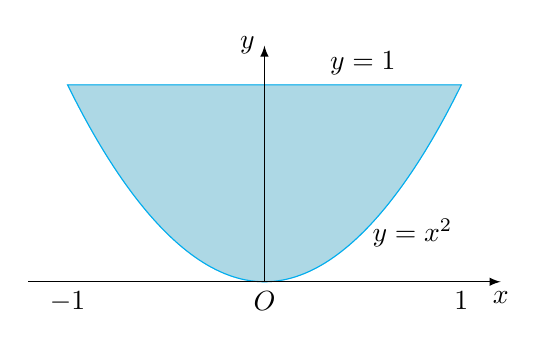
\begin{tikzpicture}[scale = 2.5]
            %画填充色块和边界线
            \filldraw[LightBlue] (-1,1) parabola bend (0,0) (1,1) -- (-1,1) -- cycle;
            \draw[cyan] (-1,1) parabola bend (0,0) (1,1) -- (-1,1) -- cycle;
            %标注边界线的表达式
            \node[right] at (0.5, 0.25) {$y=x^2$};
            \node[above] at (0.5, 1) {$y=1$};
            \node[below] at (1,0) {$1$};
            \node[below] at (-1,0) {$-1$};
            %标注坐标轴
            \draw[-latex] (0, 0) -- (0, 1.2) node[left] {$y$};
            \draw[-latex] (-1.2, 0) -- (1.2, 0) node[below] {$x$};
            \node[below] at (0,0) {$O$};
        \end{tikzpicture}
    \end{center}
    根据概率密度 $f(x,y)$ 的性质
    $$
        \int_{-\infty}^{+\infty}\int_{-\infty}^{+\infty} f(x,y) \,\mathrm{d}x\mathrm{d}y
        = \int_{-1}^1\int_{x^2}^1 cx^2y \,\mathrm{d}x\mathrm{d}y
        = c\int_{-1}^1 x^2\left(\frac{1}{2} - \frac{1}{2}x^4\right)\mathrm{d}x
        = \frac{4}{21}c
        = 1.
    $$
    解得
    $$
        c = \frac{21}{4}.
    $$
    (2) 根据边缘概率密度的定义,$X$的边缘概率密度为
    $$
        f_X(x)
        = \int_{-\infty}^{+\infty} f(x,y) \,\mathrm{d}y
        = \int_{x^2}^{1} \frac{21}{4}x^2y \,\mathrm{d}y
        = \begin{dcases}
            \frac{21}{8}x^2(1-x^4), & -1 \leqslant x \leqslant 1, \\
            0,                      & \text{其他}.
        \end{dcases}
    $$
    同理, $Y$ 的边缘概率密度为
    $$
        f_Y(y) = \int_{-\infty}^{+\infty} f(x,y) \,\mathrm{d}x
        = \int_{-\sqrt{y}}^{\sqrt{y}} \frac{21}{4}x^2y \,\mathrm{d}x
        = \begin{dcases}
            \frac{7}{2}y^{\frac{5}{2}}, & 0 \leqslant y \leqslant 1, \\
            0,                          & \text{其他}.
        \end{dcases}
    $$
\end{solution}


\begin{question}{题目11}
    以 $X$ 记某医院一天出生的婴儿的个数,$Y$ 记其中男婴的个数,设 $X$ 和 $Y$ 的联合分布律为
    $$
        P\{X=n, Y=m\} = \frac{\mathrm{e}^{-14}(7.14)^m(6.86)^{n-m}}{m!(n-m)!}
    $$
    $$
        (n = 0, 1, 2, \cdots, \quad m = 0, 1, 2, \cdots n)
    $$
    \begin{itemize}
        \item [(1)] 求边缘分布律.
        \item [(2)] 求条件分布律.
        \item [(3)] 特别,写出当 $X=20$ 时, $Y$ 的条件分布律.
    \end{itemize}
\end{question}
\begin{solution}
    (1) 根据边缘分布函数的定义,$X$ 的边缘分布函数为
    $$
        \begin{aligned}
            P\{X=n\}
             & = \sum_{m=0}^{n} \frac{\mathrm{e}^{-14}(7.14)^m(6.86)^{n-m}}{m!(n-m)!}               \\
             & = \sum_{m=0}^{n} \frac{\mathrm{e}^{-14}}{n!} \frac{n!}{m!(n-m)!}(7.14)^m(6.86)^{n-m} \\
             & = \frac{\mathrm{e}^{-14}}{n!} \sum_{m=0}^{n} C_n^m (7.14)^m(6.86)^{n-m}              \\
             & = \frac{\mathrm{e}^{-14}}{n!} (7.14+6.86)^n                                          \\
             & = \frac{14^n \mathrm{e}^{-14}}{n!}
            (n = 0, 1, 2, \cdots).
        \end{aligned}
    $$
    同理可得 $Y$ 的边缘分布函数
    $$
        \begin{aligned}
            P\{Y=m\}
             & = \sum_{n=m}^{\infty} \frac{\mathrm{e}^{-14}(7.14)^m(6.86)^{n-m}}{m!(n-m)!}           \\
             & = \frac{\mathrm{e}^{-14}(7.14)^m}{m!} \sum_{n=m}^{\infty} \frac{(6.86)^{n-m}}{(n-m)!} \\
             & = \frac{\mathrm{e}^{-14}(7.14)^m}{m!} \mathrm{e}^{6.86}                               \\
             & = \frac{(7.14)^m\mathrm{e}^{-7.14}}{m!}
            (m = 0, 1, 2, \cdots).
        \end{aligned}
    $$
    (2) 根据条件概率公式,得到 $X$ 的条件分布律
    $$
        \begin{aligned}
            P\{X=n | Y=m\}
             & = \frac{P\{X=n,Y=m\}}{P\{Y=m\}}                                                                              \\
             & = \left. \frac{\mathrm{e}^{-14}(7.14)^m(6.86)^{n-m}}{m!(n-m)!} \right/ \frac{(7.14)^m\mathrm{e}^{-7.14}}{m!} \\
             & = \frac{(6.86)^{n-m}\mathrm{e}^{-6.86}}{(n-m)!}
            (n-m = 0, 1, 2, \cdots).
        \end{aligned}
    $$
    同理,得到 $Y$ 的条件分布律
    $$
        \begin{aligned}
            P\{Y=m|X=n\}
             & = \frac{P\{X=n,Y=m\}}{P\{X=n\}}                                                                       \\
             & = \left.\frac{\mathrm{e}^{-14}(7.14)^m(6.86)^{n-m}}{m!(n-m)!} \right/ \frac{14^n\mathrm{e}^{-14}}{n!} \\
             & = \frac{n!}{m!(n-m)!}\left(\frac{7.14}{14}\right)^m\left(\frac{6.86}{14}\right)^{n-m}                 \\
             & = C_n^m(0.51)^m(0.49)^{n-m}
            (m = 0, 1, \cdots, n).
        \end{aligned}
    $$
    (3) 特别地,当 $X=30$ 时
    $$
        P\{Y=m|X=20\} = C_{20}^{m} (0.51)^m(0.49)^{20-m}
        (m = 0, 1, 2, \cdots, n).
    $$
\end{solution}


\begin{question}{题目18}
    设 $X$ 和 $Y$ 是两个相互独立的随机变量,$X$ 在区间 $(0,1)$ 上服从均匀分布,$Y$ 的概率密度为
    $$
        f_Y(y) = \begin{dcases}
            \frac{1}{2}\mathrm{e}^{-\frac{y}{2}}, & y>0,           \\
            0,                                    & y \leqslant 0.
        \end{dcases}
    $$
    \begin{itemize}
        \item [(1)] 求 $X$ 和 $Y$ 的联合概率密度.
        \item [(2)] 设有 $a$ 的二次方程为 $a^2 + 2Xa + Y = 0$,试求 $a$ 有实根的概率.
    \end{itemize}
\end{question}
\begin{solution}
    (1) 随机变量 $X$ 在区间 $(0,1)$ 上服从均匀分布,其概率密度为
    $$
        f_X(x) = \begin{cases}
            1, & 0<x<1,       \\
            0, & \text{其他}.
        \end{cases}
    $$
    由于 $X$ 和 $Y$ 相互独立,那么
    $$
        f(x,y) = f_X(x)f_Y(y) = \begin{dcases}
            \frac{1}{2}\mathrm{e}^{-\frac{y}{2}}, & 0 < x < 1, y > 0, \\
            0,                                    & \text{其他}.
        \end{dcases}
    $$
    (2) 关于 $a$ 的二次方程有实根,需满足判别式
    $$
        \Delta = 4X^2 - 4Y \geqslant 0 .
    $$
    即
    $$
        X^2 \geqslant Y
    $$
    概率密度不为零的区域如图所示
    \begin{center}
        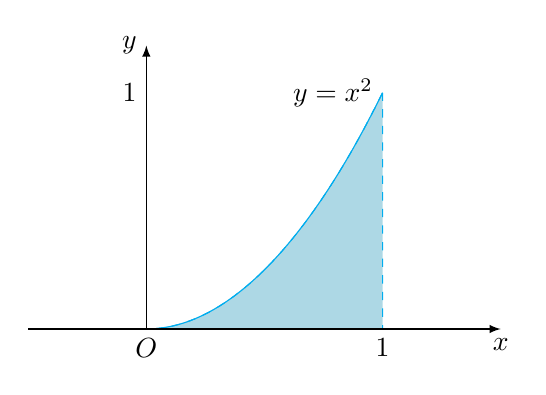
\begin{tikzpicture}[scale = 3]
            \filldraw[LightBlue] (1, 1) parabola bend (0, 0) (1, 0);
            %\draw[cyan, dashed] (1, 0) -- (1, 1);
            % \draw[cyan] (1,1) parabola bend (0,0) (1,0) -- (1,0);
            \draw[cyan, dashed] (1, 1) parabola bend (0, 0) (1,0) -- (1,1) -- cycle;
            \draw[cyan] (1, 1) parabola bend (0, 0) (1,0);
            %标注点
            \node[below] at (1,0) {$1$};
            \node[left] at (0,1) {$1$};
            \node[left] at (1, 1) {$y=x^2$};
            %标注坐标轴
            \draw[-latex] (-0.5, 0) -- (1.5, 0) node[below] {$x$};
            \draw[-latex] (0, 0) -- (0, 1.2) node[left] {$y$};
            \node[below] at (0,0) {$O$};
        \end{tikzpicture}
    \end{center}
    与之对应的概率为
    $$
        P\{X^2 \geqslant Y\}
        =\int_{-\infty}^{+\infty}\int_{-\infty}^{+\infty} f(x,y) \,\mathrm{d}x\mathrm{d}y
        = \int_{0}^{1} \mathrm{d}x \int_{0}^{x^2} \frac{1}{2}\mathrm{e}^{-\frac{y}{2}} \mathrm{d}y
        =\int_{0}^{1} 1-\mathrm{e}^{-\frac{x^2}{2}} \mathrm{d}x.
    $$
    凑出含有标准正态分布的因式
    $$
        P\{X^2 \geqslant Y\}
        = 1 - \sqrt{2\pi} \int_{0}^{1} \frac{1}{\sqrt{2\pi}} \mathrm{e}^{-\frac{x^2}{2}} \mathrm{d}x
        = 1 - \sqrt{2\pi}\left[\Phi(1)-\Phi(0)\right]
        \approx 0.1445.
    $$
    或者直接用计算器求定积分
    $$
        P\{X^2 \geqslant Y\}
        = 1 - \int_{0}^{1} \mathrm{e}^{-\frac{x^2}{2}} \mathrm{d}x
        \approx 0.1444.
    $$
\end{solution}


\begin{question}{题目24}
    设随机变量 $(X,Y)$ 的概率密度为
    $$
        f(x,y) = \begin{dcases}
            \frac{1}{2}(x+y)\mathrm{e}^{-(x+y)}, & x>0,y>0,     \\
            0,                                   & \text{其他}.
        \end{dcases}
    $$
    \begin{itemize}
        \item [(1)] 问 $X$ 和 $Y$ 是否相互独立?
        \item [(2)] 求 $Z=X+Y$ 的概率密度.
    \end{itemize}
\end{question}
\begin{solution}
    (1) 概率密度不为零的区域如图所示
    % $$
    %     G = \begin{cases}
    %         x>0, \\
    %         y>0.
    %     \end{cases}
    % $$
    \begin{center}
        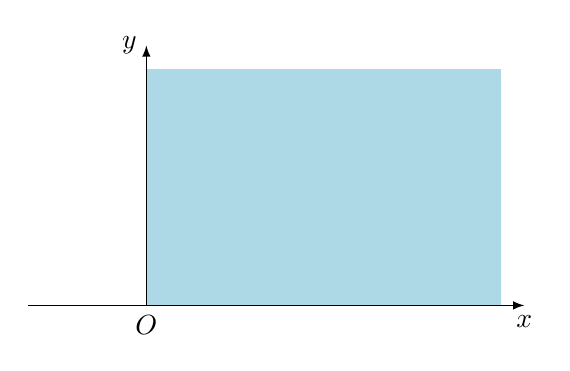
\begin{tikzpicture}[scale = 3]
            %画填充色快
            \filldraw[LightBlue] (0, 0) -- (0, 1) -- (1.5, 1) -- (1.5, 0) -- cycle;
            %标注坐标轴
            \draw[-latex] (-0.5, 0) -- (1.6, 0) node[below] {$x$};
            \draw[-latex] (0, 0) -- (0, 1.1) node[left] {$y$};
            \node[below] at (0,0) {$O$};
        \end{tikzpicture}
    \end{center}
    根据边缘概率密度的定义,$X$ 的边缘概率密度为
    $$
        \begin{aligned}
            f_X(x)
             & = \int_{-\infty}^{+\infty} f(x,y) \,\mathrm{d}y = \int_{0}^{+\infty} \frac{1}{2}(x+y)\mathrm{e}^{-(x+y)} \,\mathrm{d}y                     \\
             & = \left.-\frac{1}{2}(x+y)\mathrm{e}^{-(x+y)}\right|_{y=0}^{y=+\infty} - \int_0^{+\infty} \frac{1}{2} \mathrm{e}^{-(x+y)}\mathrm{d}[-(x+y)] \\
             & = \frac{x}{2}\mathrm{e}^{-x} - \left.\left[\frac{1}{2}\mathrm{e}^{-(x+y)}\right]\right|_{y=0}^{y=+\infty}                                  \\
             & = \frac{x}{2}\mathrm{e}^{-x} + \frac{1}{2}\mathrm{e}^{-x}.
        \end{aligned}
    $$
    即
    $$
        f_X(x) = \begin{dcases}
            \frac{\mathrm{e}^{-x}}{2}(x+1), & x>0,         \\
            0,                              & \text{其他}.
        \end{dcases}
    $$
    同理,$Y$ 的边缘概率密度为
    $$
        f_Y(y) = \int_{-\infty}^{+\infty} f(x,y) \,\mathrm{d}x
        = \begin{dcases}
            \frac{\mathrm{e}^{-y}}{2}(y+1), & y>0,         \\
            0,                              & \text{其他}.
        \end{dcases}
    $$
    由此可知
    $$
        f_X(x)f_Y(y) \neq f(x,y).
    $$
    即 $X$ 和 $Y$ 不独立.\\
    (2) 概率密度不为零的区域如图所示
    \begin{center}
        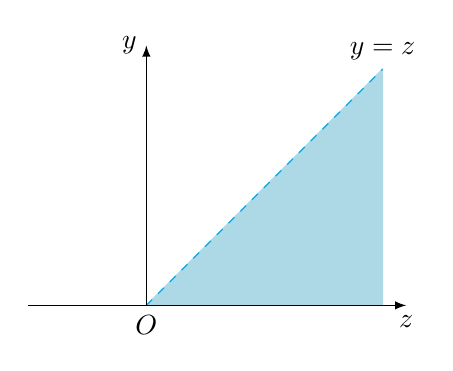
\begin{tikzpicture}[scale = 3]
            %画填充色快
            \filldraw[LightBlue] (0, 0) -- (1, 0) -- (1, 1) -- cycle;
            \draw[cyan, dashed] (0, 0) -- (1, 1);
            %画坐标系并标注
            \draw[-latex] (-0.5, 0) -- (1.1, 0) node[below] {$z$};
            \draw[-latex] (0, 0) -- (0, 1.1) node[left] {$y$};
            \node[below] at (0, 0) {$O$};
            %标注区域边界
            \node[above] at (1,1) {$y=z$};
        \end{tikzpicture}
    \end{center}
    根据两个随机变量的函数分布,$Z=X+Y$ 的概率密度可表示为
    $$
        f_Z(z) = \int_{-\infty}^{+\infty} f(z-y,y) \,\mathrm{d}y
        = \int_0^z\frac{1}{2}(z-y+y)\mathrm{e}^{-(z-y+y)}\mathrm{d}y
        %& = \begin{dcases} \frac{1}{2} \int_0^z z\mathrm{e}^{-z} \mathrm{d}y, & z-y>0, y>0, \\ 0,& \text{其他}. \end{dcases}
        = \begin{dcases}
            \frac{z^2}{2}\mathrm{e}^{-z}, & z>0,z>y      \\
            0,                            & \text{其他}.
        \end{dcases}
    $$
\end{solution}

